\section{Usability Study (BYU 2019)}

\subsection*{Overview}
\begin{frame}
  \frametitle{Usability Study (BYU 2019)}

  \begin{itemize}
    \item Conducted at Brigham Young University, Utah
    \item Two independent studies:
          \begin{enumerate}
            \item Two-week study on the use of 2FA methods
                  \begin{itemize}
                    \item Login to online banking app
                    \item 12 times over course of two weeks
                  \end{itemize}
            \item Study on the setup of different 2FA methods
          \end{enumerate}
    \item Evaluation of time and usability
  \end{itemize}
  \note{
    \begin{itemize}
      \item Two parts, day-to-day usage and only setup process
      \item day-to-day
            \begin{itemize}
              \item no remember me feature
              \item every participant only one method
            \end{itemize}
      \item setup process
            \begin{itemize}
              \item every participant sets up every method
              \item can compare it
              \item tested seperately \textrightarrow maybe only setup needs to be improved or vice versa
            \end{itemize}
    \end{itemize}
  }

\end{frame}

\subsection{Day-to-Day Use}

\begin{frame}
  \frametitle{Time to Authenticate}

  \begin{itemize}
    \item Time from successful password entry to authentification
  \end{itemize}
  \begin{figure}[c]
    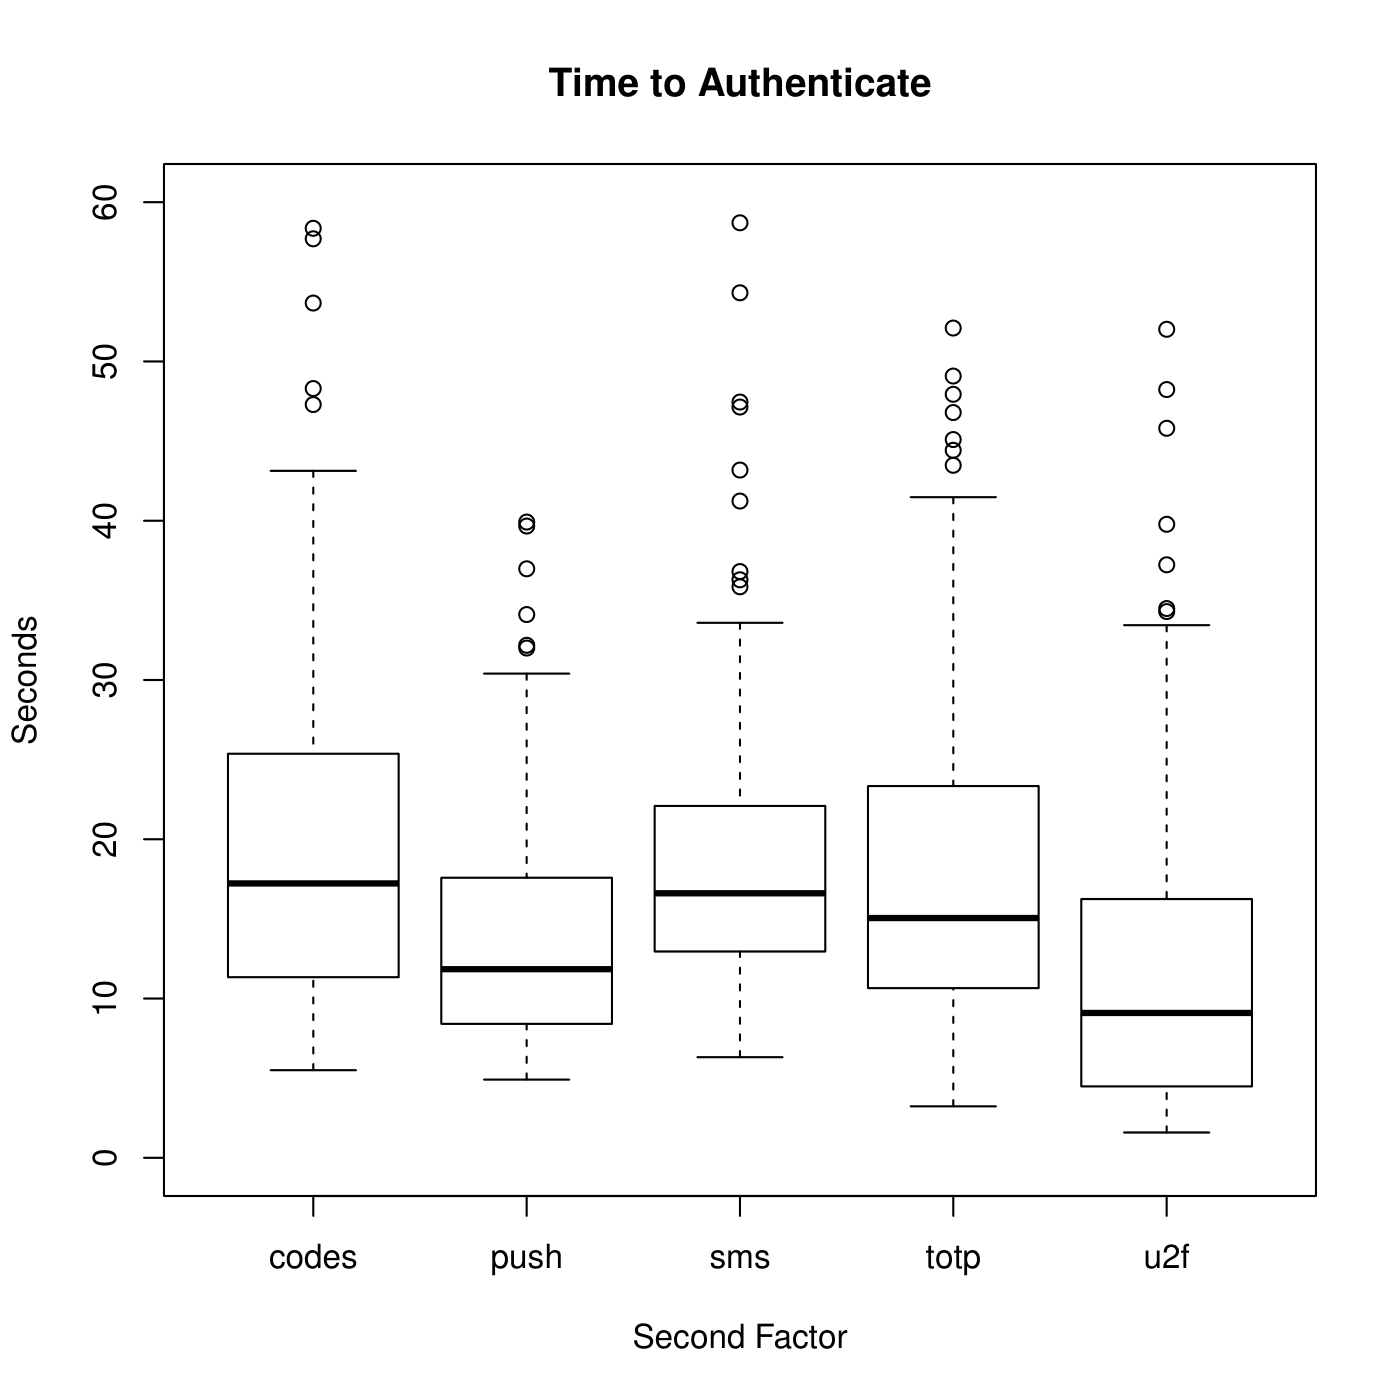
\includegraphics[height=0.8\textheight]{authentication-time}\cite{reese2019}
  \end{figure}

  \note{
    \begin{itemize}
      \item Erste betrachtete Metrik: Authentifizierungszeit
      \item Zeit, für Passwort benötigt nicht mit eingerechnet
      \item U2F am schnellsten, wahrscheinlich weil Nutzer YubiKey am Gerät stecken haben
      \item am zweitschnellsten Push-Benachrichtigungen
      \item Andere 3 Methoden: Zeit zum Eintippen der Zahlen benötigt, verlangsamt Prozess
      \item SMS: Zeit zum Versenden kommt dazu % chktex 13
      \item Codes müssen rausgesucht werden, nicht unbedingt immer zur Hand
      \item \begin{itemize}
              \item[\textrightarrow] wahrscheinlich große Varianz aufgrund von verschiedenen Aufbewahrungsmöglichkeiten
            \end{itemize}
    \end{itemize}
  }

\end{frame}

\begin{frame}
  \frametitle{Usability of Authentication}

  \begin{itemize}
    \item Assessment of perceived usability according to standard scale SUS\,
\includegraphics[height=0.25\baselineskip]{sus}
          {\tiny\textcolor{white}{\endnote{\url{https://borderpolar.com/wp-content/uploads/2021/06/red-among-us-png-842x1024.png.webp}}}} % chktex 29
  \end{itemize}
  \begin{figure}[c]
    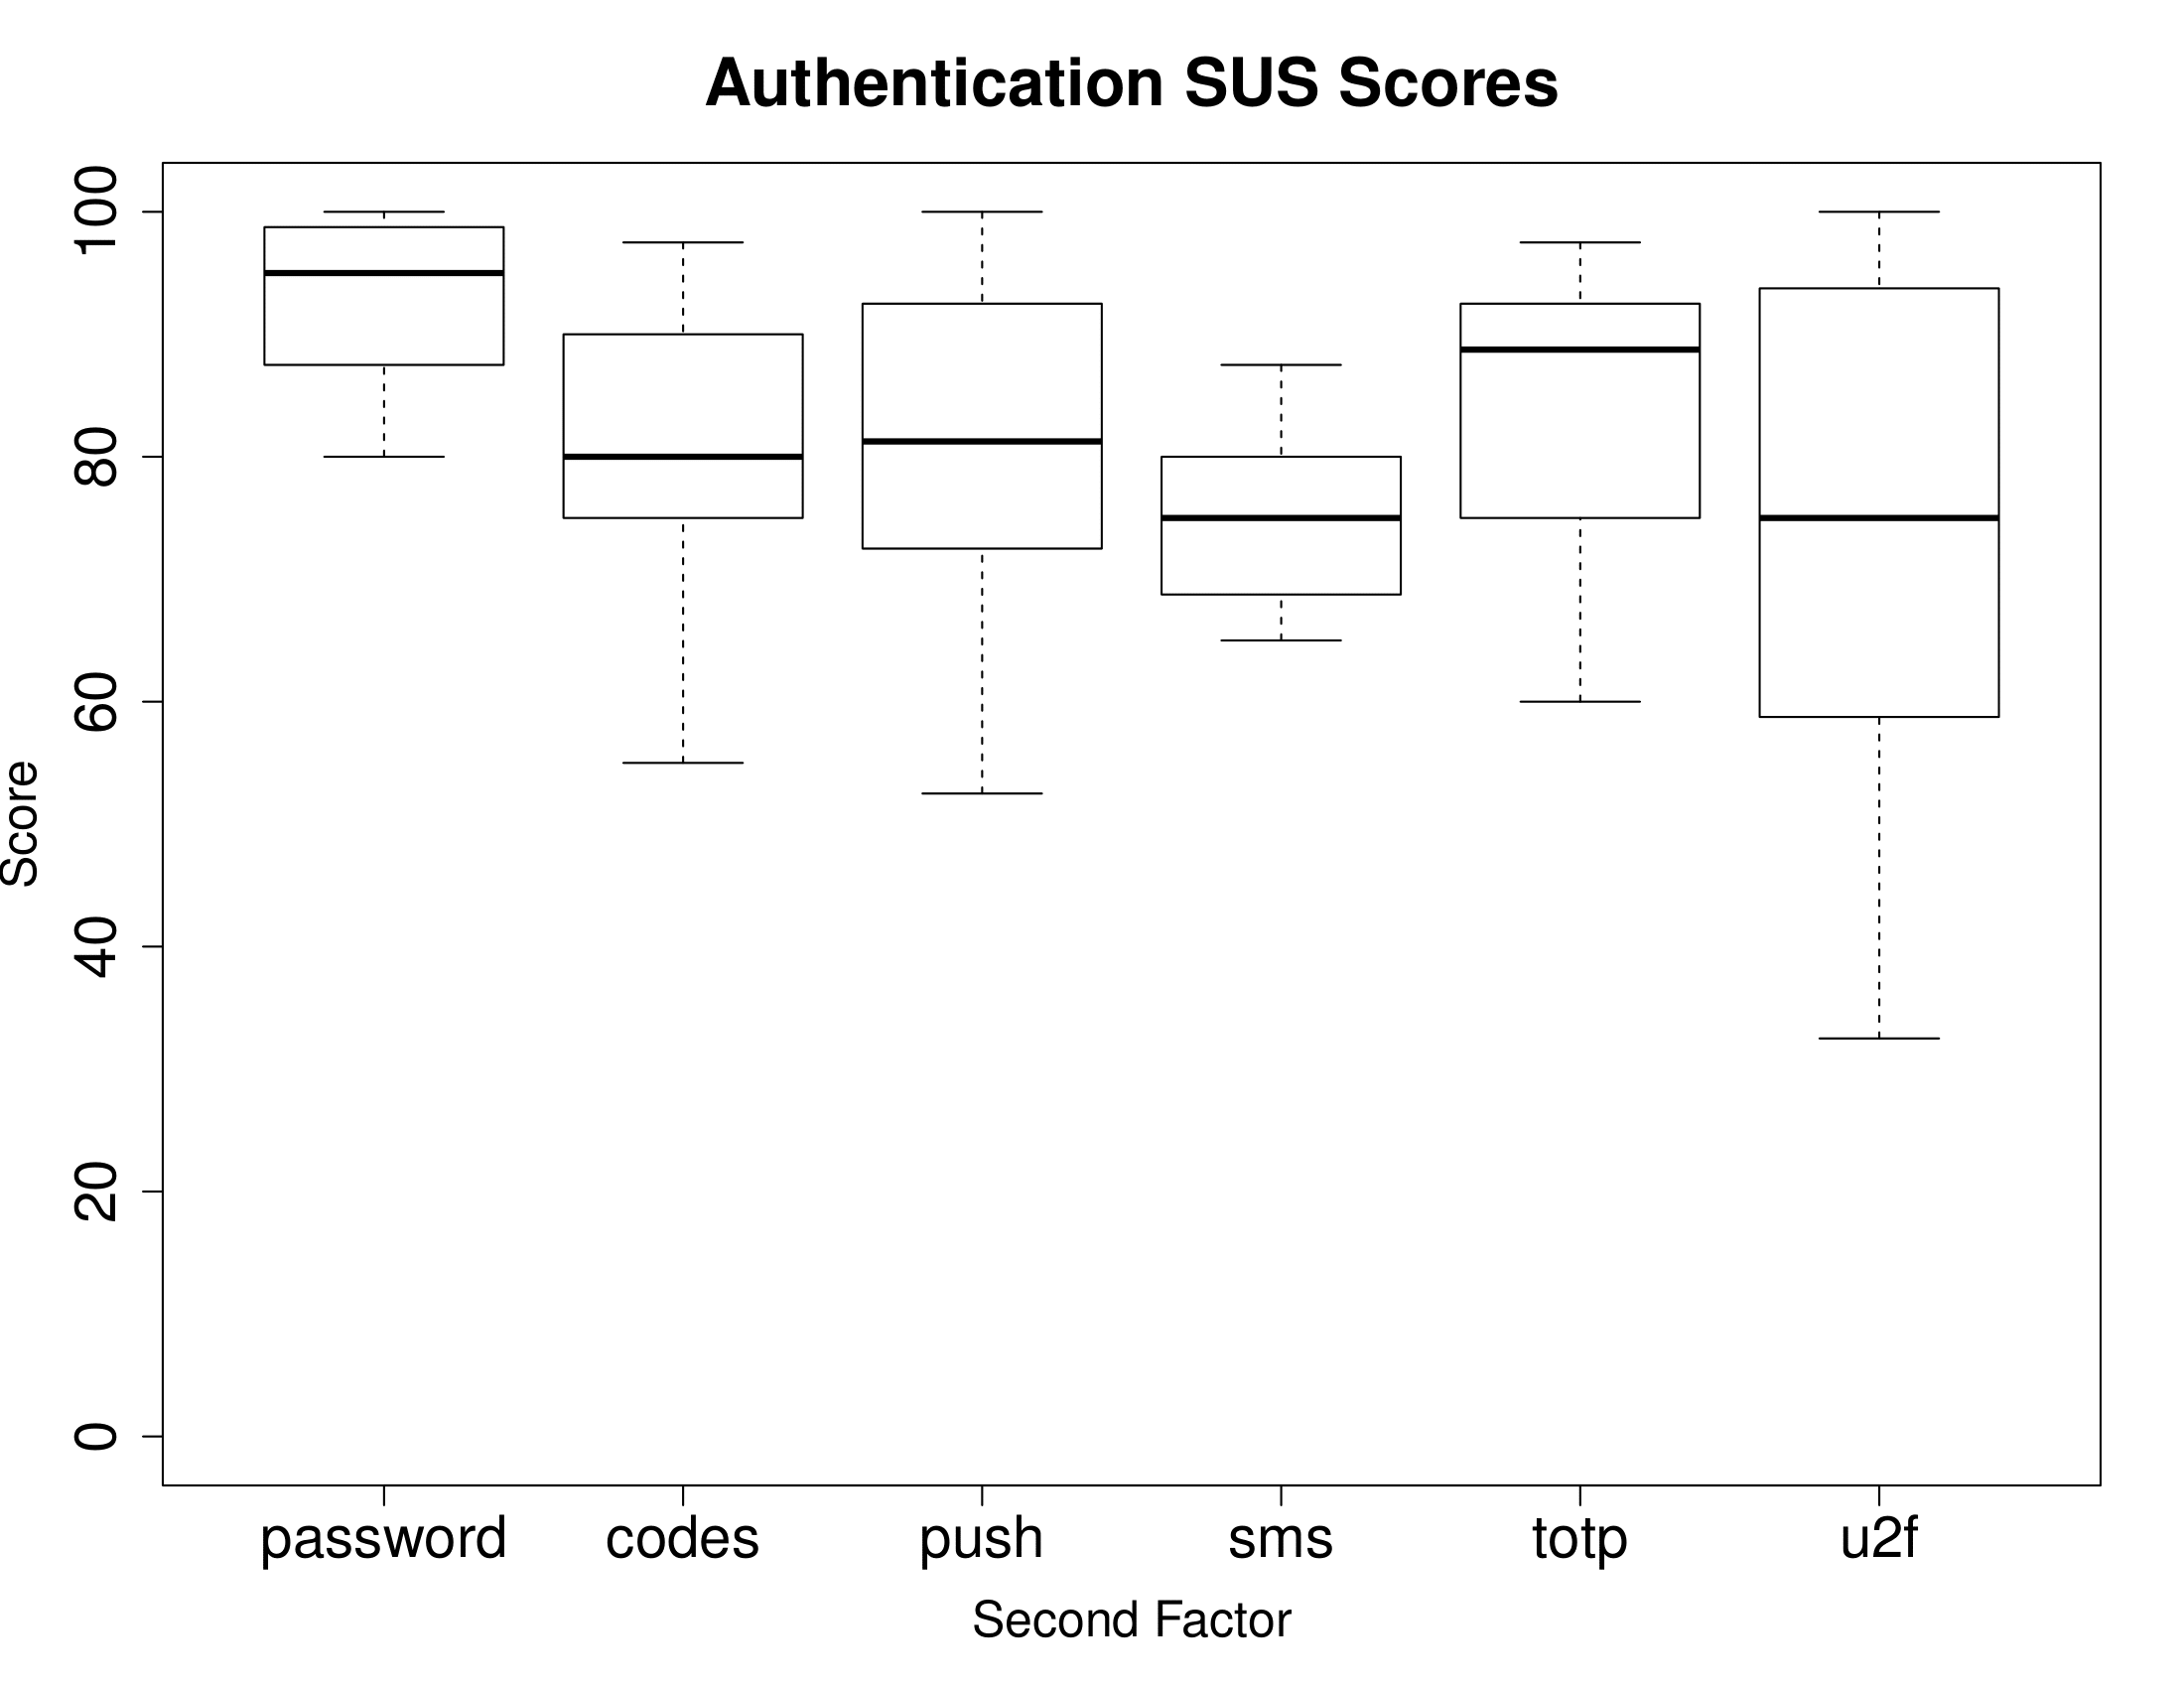
\includegraphics[height=0.76\textheight]{authentication-sus}\cite{reese2019}
  \end{figure}

  \note{
    \begin{itemize}
      \item Passwort als Kontrollwert
      \item andere Werte alle schlechter, fügen ja nur weitere Schritte hinzu
      \item obwohl TOTP am drittlangsamsten, höchster Score unter 2FA-Methoden
            \begin{itemize}
              \item Google App wurde benutzt, Implementierung wahrscheinlich nutzerfreundlich
              \item Manche Personen haben sich beschwert, dass die Codes zu schnell ablaufen zum Eingeben
              \item Erklärt auch längere Zeit aus vorheriger Folie
            \end{itemize}
      \item Auch interessant: U2F hatte sehr große Varianz, schnitt am schlechtesten ab, obwohl zeitlich am schnellsten
            \begin{itemize}
              \item Zeit nicht alles, muss auch komfortabel sein
              \item große Unterschiede durch verschiedene Möglichkeiten YubiKey aufzubewahren
              \item[\textrightarrow] nicht alle wollen extra Gerät, ist kein Handy was man so oder so hat
            \end{itemize}
    \end{itemize}
  }

\end{frame}

\subsection{Setup of 2FA}
\begin{frame}
  \frametitle{Time to Setup}

  \begin{itemize}
    \item Time between start of setup and completion
  \end{itemize}
  \begin{figure}[c]
    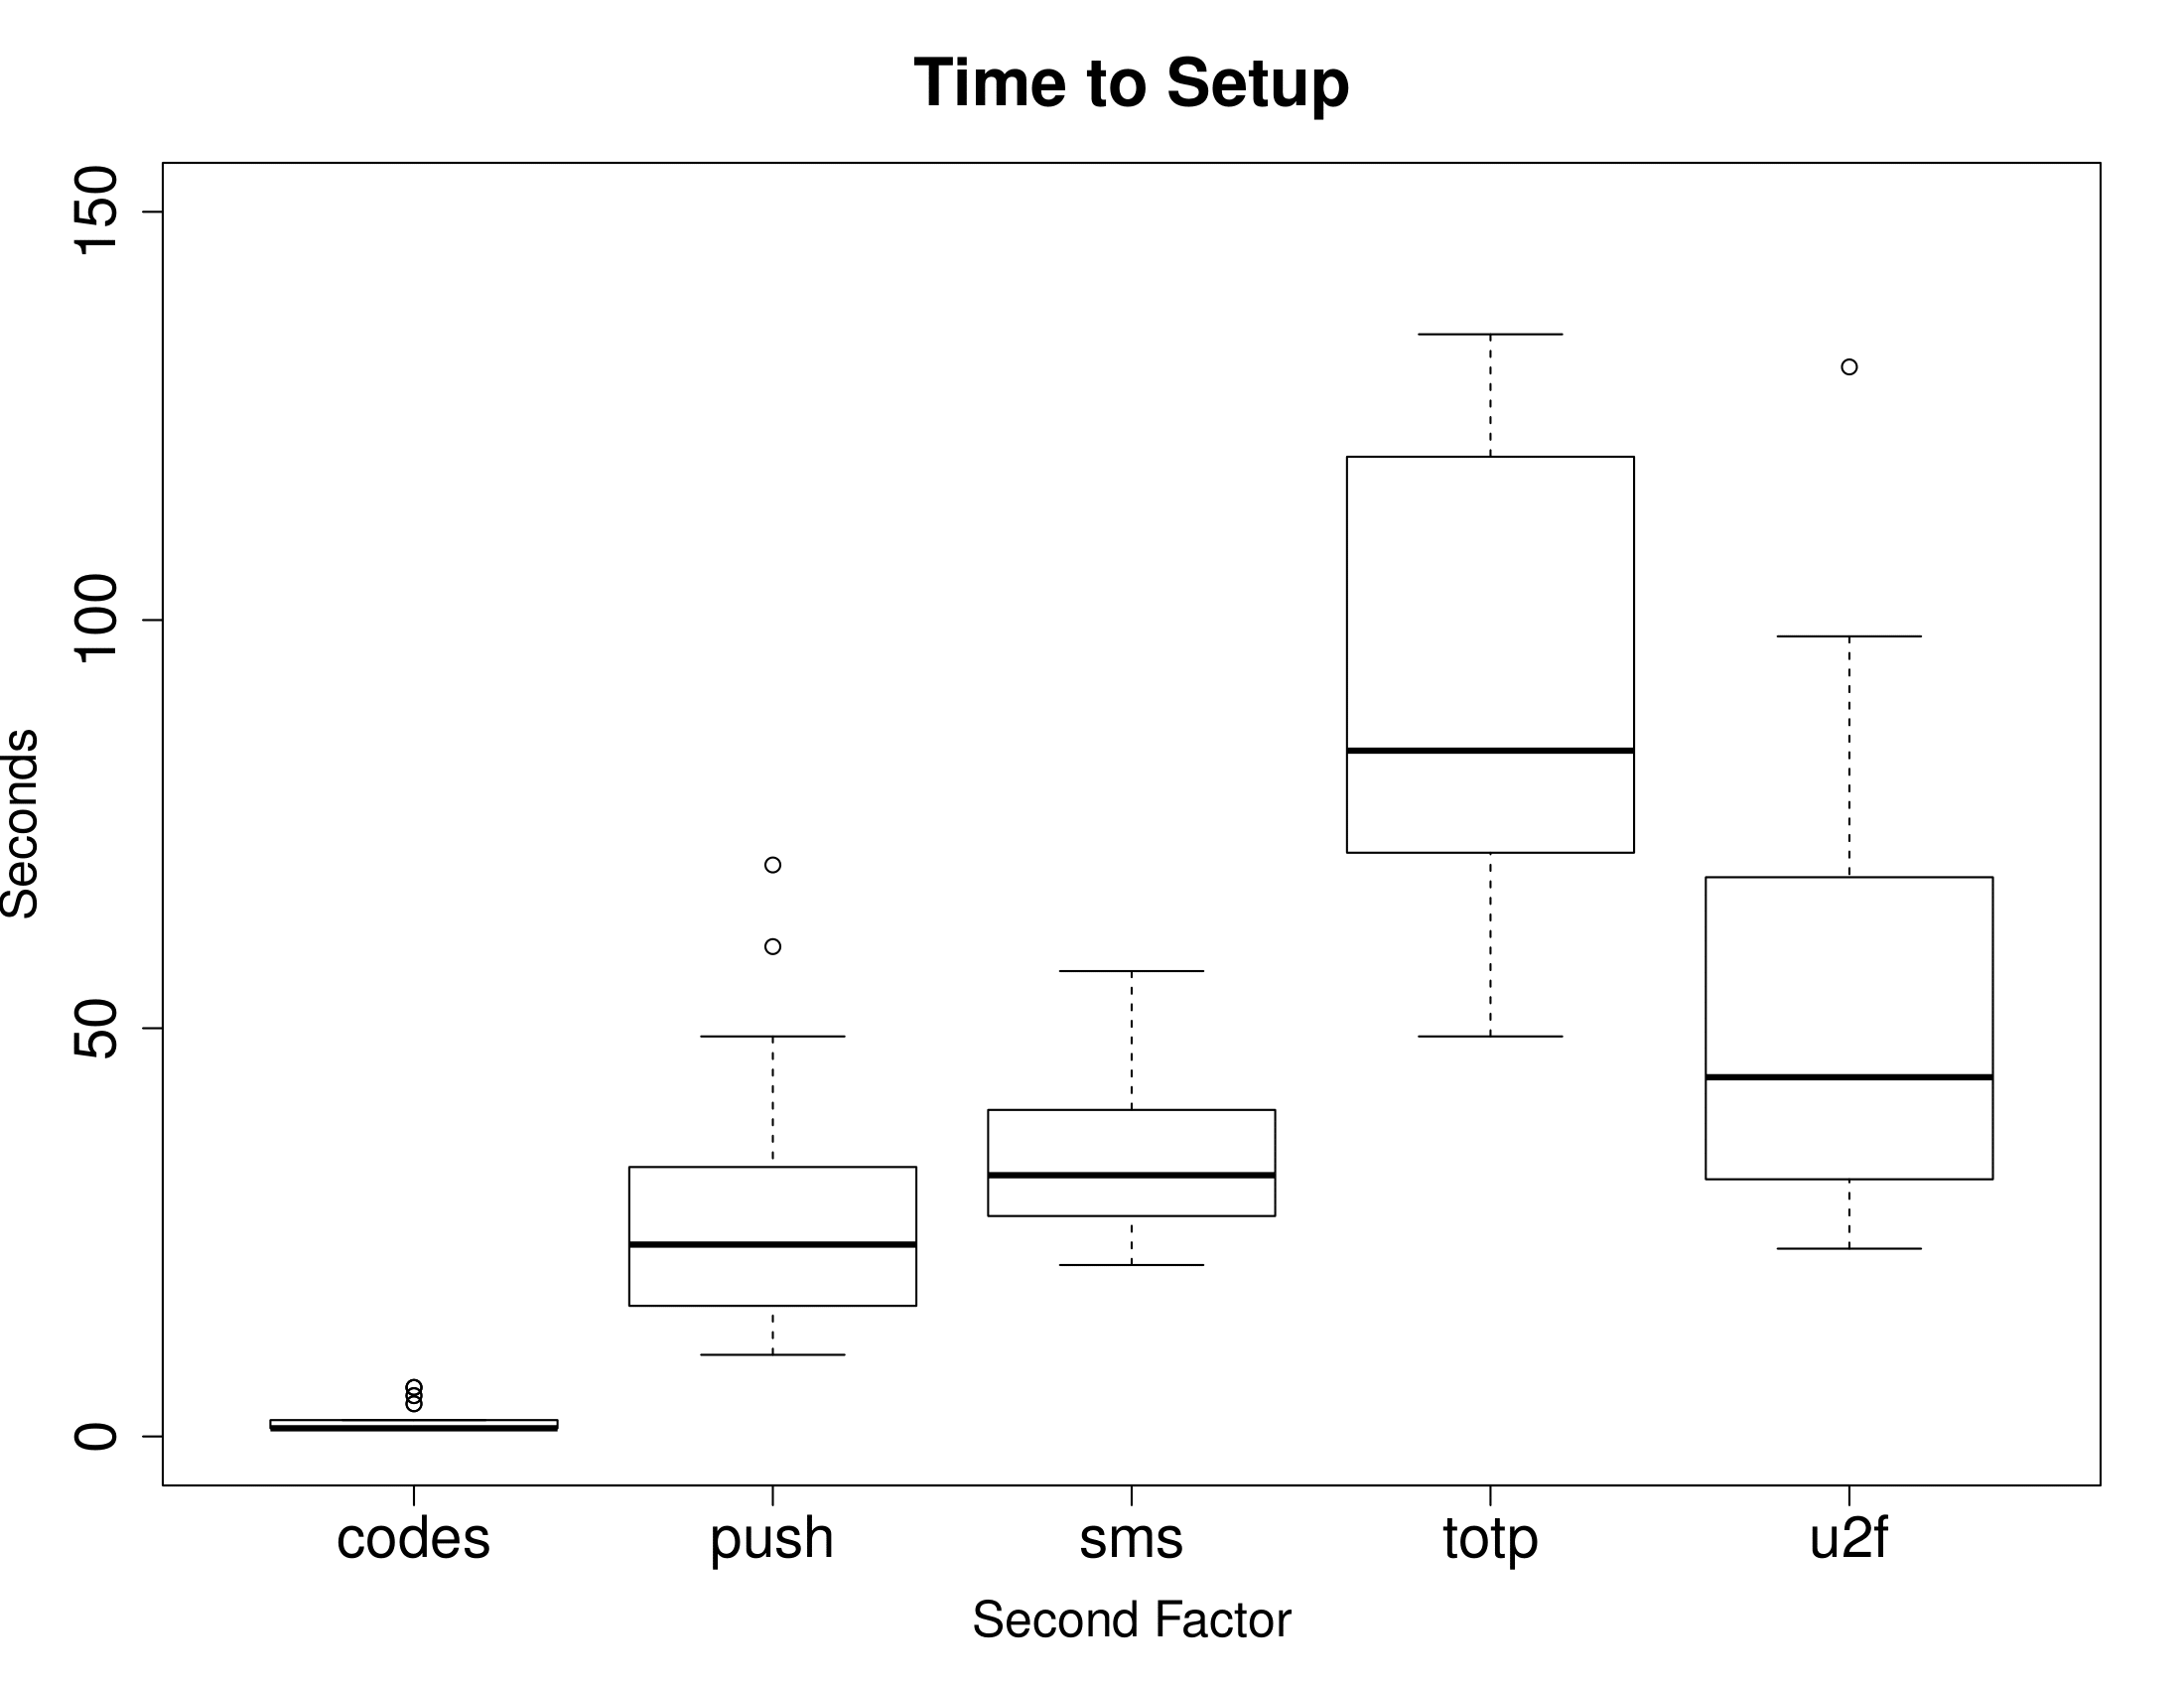
\includegraphics[height=0.8\textheight]{setup-time}\cite{reese2019}
  \end{figure}

  \note{
    \begin{itemize}
      \item Einrichtungszeit für Codes am geringsten,
            da Zeit zum Abspeichern / Ausdrucken / wie auch immer aufbewahren nicht mit betrachtet wurde
            \begin{itemize}
              \item[\textrightarrow] Zeiten wären zu unterschiedlich voneinander gewesen, da schon von Drucker abhängt
            \end{itemize}
      \item Push und SMS am zweitschnellsten, Angabe von Telefonnummer und Verbindung mit Push-App schnell
      \item TOTP und U2F hatten zwei fehlgeschlagene Einrichtungen und waren am langsamsten
      \item Langsame Einrichtung von U2F trotzdem noch bei ca.\ einer Minute
            \begin{itemize}
              \item[\textrightarrow] durch schnelle tagtägliche Benutzung vielleicht zu Entschuldigen
              \item Allerdings muss Nutzer bereits U2F Gerät wie YubiKey besitzen
            \end{itemize}
    \end{itemize}
  }

\end{frame}

\begin{frame}
  \frametitle{Setup Usability}

  \begin{itemize}
    \item Single Ease Question (SEQ), scale from 1 (very difficult) to 7 (very easy)
  \end{itemize}
  \begin{figure}[c]
    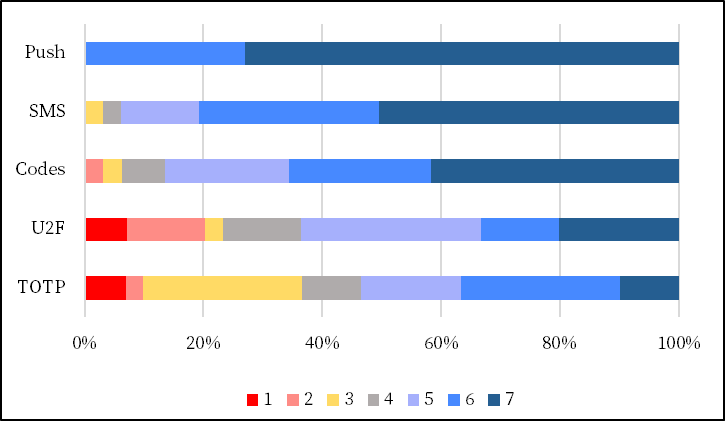
\includegraphics[height=0.7\textheight]{setup-seq}~\cite{reese2019}
  \end{figure}

  \note{
    \begin{itemize}
      \item Nutzer bewerten Usability über Single Ease Question
            \begin{itemize}
              \item Eine Frage: ``Wie Einfach war es, die Einrichtung abzuschließen?''
              \item Bewertung auf Skala von 1 bis 7, von sehr schwer bis sehr einfach
              \item Wahl von SEQ, um Ermüdung vorzubeugen, da alle Teilnehmer*innen alle Methoden eingerichtet haben
            \end{itemize}
      \item mit zeitlicher Erfassung übereinstimmend Push und SMS am einfachsten eingestuft
      \item Vermutung:
            \begin{itemize}
              \item Bekannheit von SMS verbessert Ergebnis von SMS
              \item die meisten kennen U2F und TOTP nicht, weshalb die Scores schlechter sein könnten
            \end{itemize}
    \end{itemize}
  }

\end{frame}
